% ============================================================
%  Cooperative UAV--AMR Navigation — Beamer Presentation
%  ~40 min, ~30 slides
%  Theme: Madrid | Colors: dark teal-blue
% ============================================================
\documentclass[aspectratio=169,10pt]{beamer}

% ---------- Theme & Colors ----------
\usetheme{Madrid}
\definecolor{TealDark}{RGB}{0,95,115}
\definecolor{TealLight}{RGB}{0,165,185}
\definecolor{AccentOrange}{RGB}{215,115,0}

\usecolortheme[named=TealDark]{structure}
\setbeamercolor{palette primary}   {bg=TealDark,         fg=white}
\setbeamercolor{palette secondary} {bg=TealDark!85!black, fg=white}
\setbeamercolor{palette tertiary}  {bg=TealDark!65!black, fg=white}
\setbeamercolor{palette quaternary}{bg=TealDark,         fg=white}
\setbeamercolor{frametitle}        {bg=TealDark,         fg=white}
\setbeamercolor{title}             {bg=TealDark,         fg=white}
\setbeamercolor{block title}       {bg=TealDark!90!black, fg=white}
\setbeamercolor{block body}        {bg=TealDark!8}
\setbeamercolor{alertblock title}  {bg=AccentOrange,     fg=white}
\setbeamercolor{alertblock body}   {bg=AccentOrange!12}
\setbeamercolor{alerted text}      {fg=AccentOrange}

\setbeamertemplate{navigation symbols}{}

% ---------- Packages ----------
\usepackage{amsmath,amssymb}
\usepackage{graphicx}
\usepackage{booktabs}
\usepackage{siunitx}
\sisetup{detect-all}
\usepackage{bm}
\usepackage{tikz}
\usetikzlibrary{arrows.meta,positioning,shapes.geometric}

\graphicspath{{./assets/}}

% ---------- Safe image macro ----------
% \simg[extra opts]{file} — always bounded to fit a column body
\newcommand{\simg}[2][]{\includegraphics[width=\linewidth,height=0.55\textheight,keepaspectratio,#1]{#2}}
% \simgs[extra opts]{file} — smaller, for pairs stacked in one column
\newcommand{\simgs}[2][]{\includegraphics[width=\linewidth,height=0.26\textheight,keepaspectratio,#1]{#2}}

% ---------- Presenter tag (top-right corner) ----------
% \presenter[color]{Name} — overlaid in the top-right corner; white on the
% teal frametitle bar by default, pass [TealDark] for plain/title slides.
\newcommand{\presenter}[2][white]{%
  \begin{tikzpicture}[remember picture,overlay]
    \node[anchor=north east, font=\footnotesize\bfseries, text=#1,
          xshift=-2.5mm, yshift=-1.7mm] at (current page.north east) {#2};
  \end{tikzpicture}%
  \par\vspace*{-\baselineskip}\vspace*{-\parskip}%
}

% ---------- Metadata ----------
\title[Cooperative UAV--AMR Navigation]{%
  Drone-Guided Autonomous Navigation:\\
  A Cooperative UAV--AMR System for GPS-Denied Environments}
\subtitle{Graduation Project}
\author[Ortiz \textperiodcentered{} Romo \textperiodcentered{} Rosales \textperiodcentered{} Pulido \textperiodcentered{} González]{%
  D.~Ortiz \and A.~Romo \and N.~Rosales \and S.~Pulido \and J.~González}
\institute[Tec de Monterrey]{%
  School of Engineering and Sciences\\
  Instituto Tecnológico y de Estudios Superiores de Monterrey\\[2pt]
  {\footnotesize In partnership with OMRON Automation \& Nuclea Solutions}}
\date{June 2026}

% ============================================================
\begin{document}

\begin{frame}
  \presenter[TealDark]{David}
  \titlepage
\end{frame}

\begin{frame}{Outline}
  \presenter{David}
  \tableofcontents[hideallsubsections]
\end{frame}

% ============================================================
\section{Problem \& Cooperative Approach}

\begin{frame}{Problem: Navigation Without GPS}
  \presenter{David}
  \begin{columns}[T]
    \column{0.54\textwidth}
      \textbf{Setting:} maritime ports, container yards, industrial sites
      \begin{itemize}\small
        \item GPS unreliable at ground level (multipath, blockage)
        \item No pre-built map available at mission time
        \item AMR carries \emph{no} absolute-positioning sensor by design
      \end{itemize}
      \medskip
      \textbf{Task:} navigate to a marked goal in a $4{\times}4\,\text{m}$ arena
      \begin{itemize}\small
        \item Goal pose unknown to the ground robot a priori
        \item Static obstacles; no collision allowed
        \item Map built at runtime — no prior survey
      \end{itemize}
    \column{0.43\textwidth}
      \centering
      \simg[height=0.58\textheight]{XVI_A-arena_overview_with_robots.png}\\
      {\scriptsize Test arena: AMR (floor) and UAV (above)}
  \end{columns}
\end{frame}

\begin{frame}{Cooperative Approach: UAV Surveys, AMR Navigates}
  \presenter{David}
  \centering
  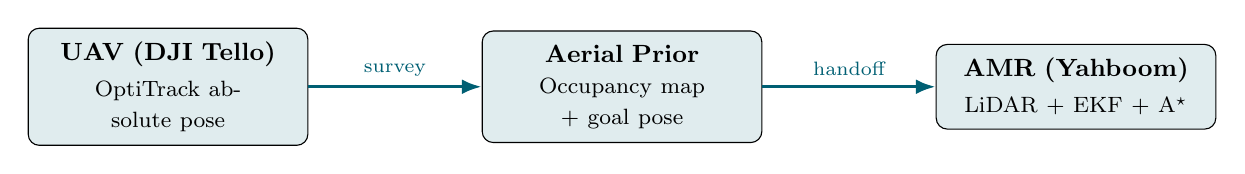
\begin{tikzpicture}[
    font=\small, node distance=6mm and 16mm,
    box/.style={draw, rounded corners, fill=TealDark!12, align=center,
                text width=3.2cm, inner sep=5pt, minimum height=10mm},
    arr/.style={-{Latex[length=2.5mm]}, very thick, TealDark}
  ]
    \node[box] (uav) {\textbf{UAV (DJI Tello)}\\[2pt]
                      \footnotesize OptiTrack absolute pose};
    \node[box, right=2.2cm of uav] (data) {\textbf{Aerial Prior}\\[2pt]
                      \footnotesize Occupancy map\\+ goal pose};
    \node[box, right=2.2cm of data] (amr) {\textbf{AMR (Yahboom)}\\[2pt]
                      \footnotesize LiDAR + EKF + A$^\star$};
    \draw[arr] (uav) -- node[above,font=\scriptsize]{survey} (data);
    \draw[arr] (data) -- node[above,font=\scriptsize]{handoff} (amr);
  \end{tikzpicture}

  \vspace{6pt}
  \begin{columns}[T]
    \column{0.46\textwidth}
      \begin{block}{UAV role}
        \begin{itemize}\small
          \item Absolute world-frame position (OptiTrack)
          \item Surveys arena $\to$ builds occupancy grid
          \item Localizes ArUco goal markers in world frame
        \end{itemize}
      \end{block}
    \column{0.46\textwidth}
      \begin{block}{AMR role}
        \begin{itemize}\small
          \item Receives aerial map + goal pose
          \item Fuses with live LiDAR map
          \item Plans A$^\star$ path; feedback-linearizing controller
        \end{itemize}
      \end{block}
  \end{columns}
\end{frame}

% ============================================================
\section{System Architecture}

\begin{frame}{Hardware Platform}
  \presenter{David}
  \begin{columns}[T]
    \column{0.36\textwidth}
      \centering
      \simgs{IV_A-AMR_and_cube.png}\\
      {\scriptsize AMR with 3D-printed ArUco cube}
      \vspace{2pt}
      \simgs{XVI_A-arena_overview_with_robots.png}\\
      {\scriptsize UAV surveying the arena}
    \column{0.60\textwidth}
      \vspace{2pt}
      {\footnotesize
      \begin{tabular}{@{}ll@{}}
        \toprule
        \textbf{Component} & \textbf{Specification} \\
        \midrule
        AMR base        & Yahboom RDK X3 (Cortex-A53) \\
        Co-processor    & Jetson Orin Nano 8\,GB + GPU \\
        LiDAR           & OraDAR MS200, $360^\circ$, \SI{15}{\hertz} \\
        Camera          & Intel RealSense D435i \\
        UAV             & DJI Tello + $45^\circ$ mirror rig \\
        UAV positioning & OptiTrack VRPN (sub-mm) \\
        \bottomrule
      \end{tabular}}
      \vspace{4pt}
      \begin{block}{Compute split}
        \small
        \textbf{RDK X3:} motor control, wheel odometry, EKF\\
        \textbf{Jetson Orin:} stitching, planning, localization, security
      \end{block}
  \end{columns}
\end{frame}

\begin{frame}{ROS 2 Node Graph}
  \presenter{Sebas}
  \centering
  \includegraphics[width=0.95\textwidth,height=0.80\textheight,keepaspectratio]{system_graph.png}\\
  \vspace{1pt}
  {\small Full ROS 2 computation graph across UAV bridge, Jetson, and RDK X3}
\end{frame}

\begin{frame}{Network Topology}
  \presenter{Sebas}
  \begin{columns}[T]
    \column{0.50\textwidth}
      \centering
      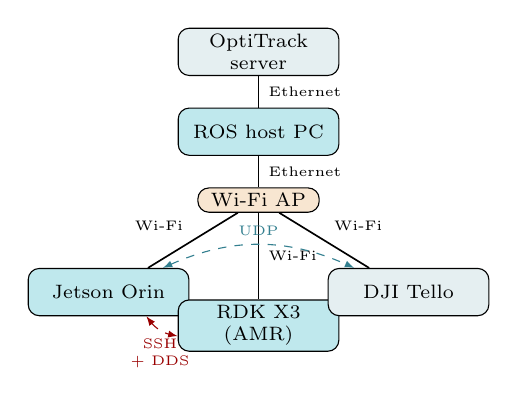
\begin{tikzpicture}[
        font=\scriptsize, node distance=4mm and 5mm,
        box/.style={draw, rounded corners, fill=TealDark!10, align=center,
                    inner sep=2pt, minimum height=6mm, text width=1.9cm},
        host/.style={draw, rounded corners, fill=TealLight!25, align=center,
                     inner sep=2pt, minimum height=6mm, text width=1.9cm},
        lnk/.style={-, semithick},
        ap/.style={draw, fill=AccentOrange!18, rounded corners,
                   align=center, inner sep=2pt, text width=1.4cm}
      ]
        \node[box]  (opti)  {OptiTrack server};
        \node[host, below=of opti]  (rospc) {ROS host PC};
        \node[ap,   below=of rospc] (apn)   {Wi-Fi AP};
        \node[host, below left=7mm and 1mm of apn] (jetson) {Jetson Orin};
        \node[host, below=11mm of apn]             (rdk)    {RDK X3 (AMR)};
        \node[box,  below right=7mm and 1mm of apn](tello)  {DJI Tello};
        \draw[lnk] (opti) -- node[right,font=\tiny]{Ethernet} (rospc);
        \draw[lnk] (rospc) -- node[right,font=\tiny]{Ethernet} (apn);
        \draw[lnk] (apn) -- node[above left,font=\tiny]{Wi-Fi} (jetson);
        \draw[lnk] (apn) -- node[right,font=\tiny]{Wi-Fi} (rdk);
        \draw[lnk] (apn) -- node[above right,font=\tiny]{Wi-Fi} (tello);
        \draw[{Latex[length=1.2mm]}-{Latex[length=1.2mm]}, dashed, red!60!black]
           (jetson) to[bend right=20]
           node[below,font=\tiny,align=center]{SSH\\+ DDS} (rdk);
        \draw[{Latex[length=1.2mm]}-{Latex[length=1.2mm]}, dashed, TealDark!80]
           (jetson) to[bend left=24]
           node[above,font=\tiny]{UDP} (tello);
      \end{tikzpicture}
    \column{0.47\textwidth}
      \vspace{4pt}
      \begin{block}{Two communication planes}
        \small
        \textbf{Control:} SSH (Paramiko) — Jetson manages RDK X3 lifecycle\\[3pt]
        \textbf{Data:} ROS 2 DDS over Wi-Fi\\
        Tello bridged over proprietary UDP SDK\\
        OptiTrack via VRPN
      \end{block}
      \vspace{4pt}
      \begin{alertblock}{Latched QoS (NFR-9)}
        \small Map and goal topics use \texttt{TRANSIENT\_LOCAL} — late-joining nodes still receive them
      \end{alertblock}
  \end{columns}
\end{frame}

% ============================================================
\section{Mission Pipeline}

\begin{frame}{12-Stage Mission FSM}
  \presenter{Sebas}
  \begin{columns}[T]
    \column{0.58\textwidth}
      \centering
      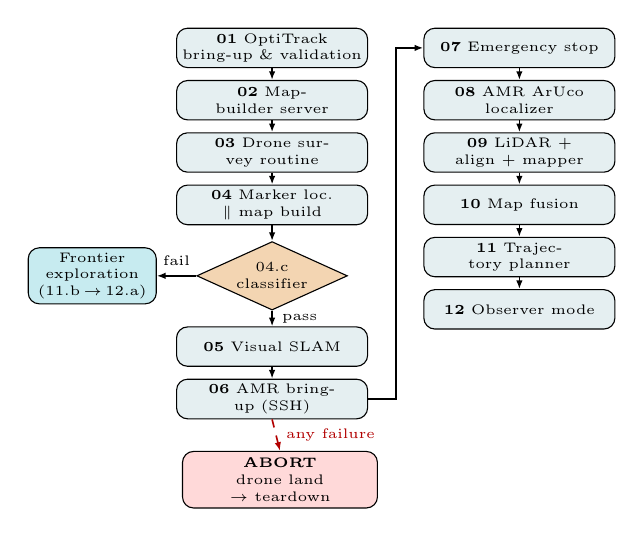
\begin{tikzpicture}[
        font=\tiny,
        stage/.style={draw, rounded corners, fill=TealDark!10, align=center,
                      text width=2.3cm, inner sep=1.8pt, minimum height=5mm},
        dec/.style={draw, diamond, aspect=2.2, fill=AccentOrange!30, align=center,
                    inner sep=0pt, text width=1.2cm},
        term/.style={draw, rounded corners, fill=red!15, align=center,
                     text width=2.3cm, inner sep=2.5pt},
        arr/.style={-{Latex[length=1.1mm]}, semithick},
        fb/.style={draw, rounded corners, fill=TealLight!22, align=center,
                   text width=1.5cm, inner sep=1.8pt}
      ]
        % left column 01..06
        \node[stage] (s1) {\textbf{01} OptiTrack bring-up \& validation};
        \node[stage, below=1.5mm of s1] (s2) {\textbf{02} Map-builder server};
        \node[stage, below=1.5mm of s2] (s3) {\textbf{03} Drone survey routine};
        \node[stage, below=1.5mm of s3] (s4) {\textbf{04} Marker loc.\ $\parallel$ map build};
        \node[dec,   below=2mm of s4]   (cls){04.c classifier};
        \node[stage, below=2mm of cls]  (s5) {\textbf{05} Visual SLAM};
        \node[stage, below=1.5mm of s5] (s6) {\textbf{06} AMR bring-up (SSH)};
        % right column 07..12
        \node[stage, right=7mm of s1] (s7)  {\textbf{07} Emergency stop};
        \node[stage, below=1.5mm of s7] (s8) {\textbf{08} AMR ArUco localizer};
        \node[stage, below=1.5mm of s8] (s9) {\textbf{09} LiDAR + align + mapper};
        \node[stage, below=1.5mm of s9] (s10){\textbf{10} Map fusion};
        \node[stage, below=1.5mm of s10](s11){\textbf{11} Trajectory planner};
        \node[stage, below=1.5mm of s11](s12){\textbf{12} Observer mode};
        % fallback branch off the 04.c classifier
        \node[fb, left=5mm of cls] (front)
              {Frontier exploration (11.b\,$\to$\,12.a)};
        % spines (cls$\to$s5 drawn separately to label the pass branch)
        \foreach \a/\b in {s1/s2,s2/s3,s3/s4,s4/cls,s5/s6}
          \draw[arr](\a)--(\b);
        \foreach \a/\b in {s7/s8,s8/s9,s9/s10,s10/s11,s11/s12}
          \draw[arr](\a)--(\b);
        \draw[arr] (cls) -- node[right,font=\tiny]{pass} (s5);
        \draw[arr] (cls) -- node[above,font=\tiny]{fail} (front);
        \draw[arr] (s6.east) -- ++(3.5mm,0) |- (s7.west);
        % abort sink
        \node[term, below=4mm of s6, xshift=1mm] (ab)
          {\textbf{ABORT}\\drone land $\to$ teardown};
        \draw[arr, dashed, red!70!black] (s6.south) -- (ab.north)
          node[midway,right,font=\tiny]{any failure};
      \end{tikzpicture}
    \column{0.40\textwidth}
      \vspace{4pt}
      \begin{block}{Key design}
        \small Stages advance on \texttt{success} only\\
        Any failure $\to$ single ABORT sink\\
        Abort: land drone first, then teardown
      \end{block}
      \vspace{4pt}
      \begin{alertblock}{Stage 04.c: map-quality branch}
        \small \textbf{PASS} $\to$ drone map + goal pose\\[2pt]
        \textbf{FAIL} $\to$ border template; arm frontier-exploration fallback
      \end{alertblock}
      \vspace{4pt}
      \begin{block}{Concurrency}
        \small Map build $\parallel$ marker localization\\
        Wall-clock: $\max(T_\text{stitch},\,T_\text{PnP})$
      \end{block}
  \end{columns}
\end{frame}

% ============================================================
\section{UAV Flight Control}

\begin{frame}{UAV: PID Controller + Boustrophedon Survey}
  \presenter{Noé}
  \begin{columns}[T]
    \column{0.54\textwidth}
      World-frame PID with feedforward and anti-windup:
      \[v_x^W = -k_{p}e_x - k_{d}\tilde{v}_x - k_{i}I_x + v_{ff,x}\]
      Body-frame rotation (Tello accepts body-frame only):
      \[\begin{pmatrix}v_x^B\\v_y^B\end{pmatrix}
        = \begin{pmatrix}\cos\psi & \sin\psi\\ -\sin\psi & \cos\psi\end{pmatrix}
          \begin{pmatrix}v_x^W\\v_y^W\end{pmatrix}\]
      \textbf{Survey:} arc-length cubic spline, zero endpoint velocities\\[3pt]
      \textbf{Fault detector:} sliding-window bad-sample ratio\\
      $\hat\rho_k = \frac{1}{W}\sum_j b_j > \rho_\text{thr}$ — handles alternating-ghost dropouts
    \column{0.43\textwidth}
      \begin{block}{Deployed gains}
        \centering\footnotesize
        \begin{tabular}{lll}
          \toprule
          Param & Value & \\
          \midrule
          $k_{p}$ & $2.0,\,2.0,\,3.0$ & (x,y,z)\\
          $k_{d}$ & $0.1,\,0.1,\,0.3$ & \\
          $k_{i}$ & $0,\,0,\,0.1$     & \\
          $v_\text{max}$ & \SI{0.6}{\meter\per\second} & \\
          \bottomrule
        \end{tabular}
      \end{block}
      \vspace{4pt}
      \textbf{6-state flight FSM}\\
      {\footnotesize pre-flight $\to$ takeoff $\to$ stabilize $\to$ \textbf{trajectory} $\to$ return $\to$ land\\
      + fault-land reachable from stabilize/trajectory/return}
  \end{columns}
\end{frame}

\begin{frame}{UAV Tracking Results}
  \presenter{Noé}
  \begin{columns}[T]
    \column{0.46\textwidth}
      \centering
      \simg[height=0.62\textheight]{VI_D-drone_trajectory_following-new.png}\\
      {\small Commanded vs.\ measured $xy$ path}
    \column{0.52\textwidth}
      \centering
      \simg[height=0.42\textheight]{VI_D-drone_trajectory_error_per_axis-new.png}\\
      {\small Per-axis absolute tracking error}
      \vspace{0pt}
      \begin{block}{Error statistics}
        \centering\scriptsize
        \begin{tabular}{lccc}
          \toprule
          Axis & Mean $|e|$ & RMS & Peak \\
          \midrule
          $x$ & 3.8\,cm & 4.4\,cm & 14.3\,cm\\
          $y$ & 2.3\,cm & 2.8\,cm & 7.6\,cm\\
          $z$ & 3.1\,cm & 3.7\,cm & 10.6\,cm\\
          \bottomrule
        \end{tabular}
      \end{block}
      {\scriptsize Peak excursions at turn points; within stitching overlap margin}
  \end{columns}
\end{frame}

% ============================================================
\section{Aerial Mapping \& Image Stitching}

\begin{frame}{Similarity Transform — Not Full Homography}
  \presenter{David}
  \begin{columns}[T]
    \column{0.55\textwidth}
      \textbf{Full homography} (8 DOF): over-parameterized
      \begin{itemize}\small
        \item Arena has repetitive blue-tape grid
        \item Extra DOF let RANSAC match tape junctions $\to$ ``fan'' artifacts
      \end{itemize}
      \smallskip
      \textbf{Similarity transform} (4 DOF): translation + rotation + scale
      \[\mathbf{H}_\text{sim}=
        \begin{pmatrix}a & -b & t_x\\ b & a & t_y\\ 0 & 0 & 1\end{pmatrix},
        \quad a=s\cos\theta\]
      \begin{itemize}\small
        \item Exact model for nadir camera over a flat plane
        \item Stable across hundreds of frames
        \item \texttt{estimateAffinePartial2D} + RANSAC
      \end{itemize}
      \textbf{Matching:} $k$-NN $\to$ Lowe ratio ($r{=}0.65$) $\to$
      mutual cross-check $\to$ MAD pre-filter $\to$ RANSAC
    \column{0.42\textwidth}
      \centering
      \simgs[height=0.30\textheight]{VII_D-contour_background_mask.png}\\
      {\small HSV blue-tape exclusion mask}
      \vspace{3pt}
      \simgs[height=0.30\textheight]{VII_D-masked_stitching_final.png}\\
      {\small Masked incremental stitch}
  \end{columns}
\end{frame}

\begin{frame}{Stitching Pipeline Results}
  \presenter{David}
  \begin{columns}[T]
    \column{0.46\textwidth}
      \centering
      \simgs[height=0.30\textheight]{VII_D-final_stitching_map.png}\\
      {\small Final stitched arena map}
      \vspace{3pt}
      \simgs[height=0.30\textheight]{VII_D-transfer_on_grid.png}\\
      {\small Obstacle transfer on occupancy grid}
    \column{0.52\textwidth}
      \textbf{Obstacle consistency scoring}
      \[c = \frac{w_A s_A + w_B s_B + w_C s_C}{w_A + w_B + w_C}\]
      {\footnotesize
        $s_A$: centroid agreement,\; $s_B$: area ratio,\; $s_C$: perturbation stability\\[2pt]
        $w_A,w_B,w_C$: fixed weights of each sub-score $=(0.45,\,0.25,\,0.30)$}
      \smallskip

      Low-confidence obstacles $\to$ wider cautionary halos
      \vspace{4pt}
      \begin{block}{Memory budget (NFR-5)}
        \footnotesize
        ROI warping + $8000{\times}8000$ pre-allocated canvas\\
        Peak working set ${\approx}\,287\,\text{MB}$ on Jetson
      \end{block}
  \end{columns}
\end{frame}

\begin{frame}{Map-Quality Classifier}
  \presenter{David}
  \begin{columns}[T]
    \column{0.50\textwidth}
      \centering
      \simg[height=0.74\textheight]{VII_D-random_forest_feature_importance.png}\\
      {\small Random Forest feature importance (46 features)}
    \column{0.47\textwidth}
      \begin{itemize}\small
        \item 46 diagnostic features per map-build run
        \item Random Forest, 50-iter search, 5-fold CV; optimizes PR-AUC
        \item Inference: pure NumPy (no scikit-learn at runtime)
      \end{itemize}
      \vspace{4pt}
      \begin{alertblock}{Asymmetric cost}
        \small \textbf{False positive} (accept bad map) is worse than false negative (frontier exploration)\\[2pt]
        Threshold tuned to target precision on \texttt{pass}
      \end{alertblock}
      \vspace{4pt}
      {\footnotesize Top features: stitching residuals, green-mask wall coverage, blob statistics — physically meaningful predictors}
  \end{columns}
\end{frame}

% ============================================================
\section{Aerial Marker Localization}

\begin{frame}{ArUco Localization: Transform Chain + PnP}
  \presenter{David}
  % equation + TikZ across full width, then split below
  \textbf{Four-link transform chain:}\quad
  $T_{\text{map}\leftarrow\text{mk}}
    = T_{m\leftarrow o}\; T_{o\leftarrow d}(t)\; T_{d\leftarrow c}\; T_{c\leftarrow mk}(t)$
  \vspace{4pt}

  \begin{center}
  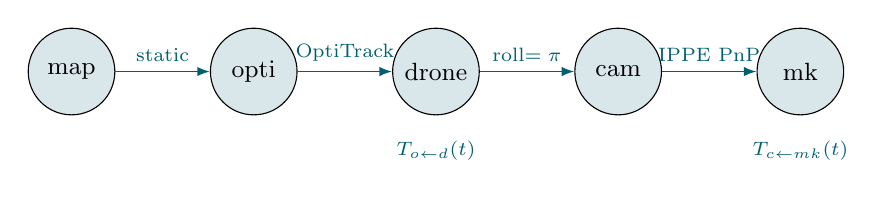
\begin{tikzpicture}[
    font=\small, node distance=12mm,
    frm/.style={draw, circle, fill=TealDark!15, inner sep=1pt, minimum size=11mm},
    tf/.style={-{Latex[length=1.6mm]}, semithick, TealDark}
  ]
    \node[frm](map){map};
    \node[frm,right=of map](opti){opti};
    \node[frm,right=of opti](drone){drone};
    \node[frm,right=of drone](cam){cam};
    \node[frm,right=of cam](mk){mk};
    \draw[tf](map)--node[above]{\scriptsize static}(opti);
    \draw[tf](opti)--node[above]{\scriptsize OptiTrack}(drone);
    \draw[tf](drone)--node[above]{\scriptsize roll$=\pi$}(cam);
    \draw[tf](cam)--node[above]{\scriptsize IPPE PnP}(mk);
    \node[below=2mm of drone,font=\scriptsize,text=TealDark]{$T_{o\leftarrow d}(t)$};
    \node[below=2mm of mk,font=\scriptsize,text=TealDark]{$T_{c\leftarrow mk}(t)$};
  \end{tikzpicture}
  \end{center}
  \vspace{4pt}

  \begin{columns}[T]
    \column{0.40\textwidth}
      \centering
      \simg[height=0.40\textheight]{VIII_A-tello_drone_detecting_aruco.png}\\
      {\scriptsize UAV in nadir view via $45^\circ$ mirror}
    \column{0.57\textwidth}
      \begin{itemize}\small
        \item \textbf{IPPE\_SQUARE:} closed-form planar PnP; two-candidate ambiguity resolved by reprojection error ($<\SI{4}{px}$)
        \item \textbf{Robust aggregation} (120--180 obs./marker):\\
              MAD gate ($k{=}3.5$) $\to$ Weiszfeld geometric median (breakdown ${\sim}50\%$) $\to$ circular median for yaw
        \item Position from stitcher (metric pixel); orientation from PnP (unaffected by map-origin shifts)
      \end{itemize}
  \end{columns}
\end{frame}

% ============================================================
\section{AMR State Estimation: EKF}

\begin{frame}{Extended Kalman Filter: 5-State Unicycle}
  \presenter{Noé}
  \begin{columns}[T]
    \column{0.50\textwidth}
      \textbf{State:} $\mathbf{X}=[x,\;y,\;\theta,\;v,\;\omega]^\top$
      {\footnotesize\[f(\mathbf{X})=\bigl[x+T_s v\cos\theta,\;y+T_s v\sin\theta,\;
                          \theta+T_s\omega,\;v,\;\omega\bigr]^\top\]}
      $Q=\mathrm{diag}(10^{-4},10^{-4},10^{-4},0.05,0.05)$\\[4pt]
      \textbf{Three sequential updates per step:}\\[2pt]
      {\footnotesize
      \begin{tabular}{@{}lll@{}}
        Wheel encoder & $(v,\omega)$ & $R_\text{wh}=\mathrm{diag}(0.2,0.2)$ \\
        IMU gyro & $\omega$ & $R_\text{imu}=0.001$ \\
        VIO $v_x$ & $v$ & $R_\text{vio}=0.1$ \\
      \end{tabular}}\\[4pt]
      Joseph-form covariance update (preserves PSD)
    \column{0.47\textwidth}
      \begin{alertblock}{The VIO problem}
        \small cuVSLAM back-end \emph{loop closures} inject velocity impulses:
        $|v_x^\text{raw}| \approx \SI{4.9}{\meter\per\second}$
        vs.\ true cruise ${\sim}\SI{0.2}{\meter\per\second}$
      \end{alertblock}
      \vspace{4pt}
      \begin{block}{Design choices}
        \small Only forward velocity \emph{scalar} fused\\
        VIO position discarded (drifts and jumps)\\[3pt]
        Implemented \textbf{from scratch} (NFR-1)
      \end{block}
  \end{columns}
\end{frame}

\begin{frame}{Adaptive VIO Gate (\texttt{ema\_gate})}
  \presenter{David}
  \begin{columns}[T]
    \column{0.50\textwidth}
      \textbf{P0:} hard clip at $|v_x|>\SI{0.5}{\meter\per\second}$\\[4pt]
      \textbf{P1:} EMA mean/variance tracking:
      \[\hat\mu_k = \alpha v_k+(1-\alpha)\hat\mu_{k-1},\quad
        \tau_k = \max(2\hat\sigma_k,\;0.17)\]
      Burst mode: spike fraction $>0.30$ in 10-sample window
      $\to$ hold \texttt{last\_good}
      \vspace{4pt}
      \centering
      \simgs[height=0.40\textheight]{IX_D-vio_raw_vs_gated.png}\\
      {\scriptsize Raw cuVSLAM, OptiTrack truth, and gate output}
    \column{0.47\textwidth}
      \centering
      \simgs[height=0.52\textheight]{IX_D-vio_gate_ablation.png}\\
      {\small Filter ablation over a loop-closure burst}
      \vspace{3pt}
      \begin{block}{Why not Butterworth LPF?}
        \footnotesize The LPF rings in response to spikes — transient propagates a sustained deviation. \texttt{ema\_gate} holds flat, close to truth.
      \end{block}
  \end{columns}
\end{frame}

\begin{frame}{EKF Results: 88\,\% Reduction in Position Error}
  \presenter{Noé}
  \begin{columns}[T]
    \column{0.49\textwidth}
      \centering
      \simg[height=0.50\textheight]{IX_D-amr_trajectory_tracking-new.png}\\
      {\small $xy$ trajectory: truth, EKF, wheel odometry}
    \column{0.49\textwidth}
      \centering
      \simg[height=0.50\textheight]{IX_D-amr_trajectory_error-new.png}\\
      {\small Absolute position error vs.\ OptiTrack}
  \end{columns}
  \vspace{3pt}
  \begin{columns}
    \column{0.50\textwidth}
      \begin{block}{}
        \centering\footnotesize
        \begin{tabular}{@{}lcc@{}}
          \toprule
          & \textbf{EKF} & \textbf{Wheel only} \\
          \midrule
          Mean $|e_x|$ & 4.6\,cm  & 52.3\,cm \\
          Mean $|e_y|$ & 6.3\,cm  & 41.6\,cm \\
          \bottomrule
        \end{tabular}
      \end{block}
    \column{0.48\textwidth}
      \centering
      {\large\color{TealDark}\bfseries ${\sim}88\%$ reduction}\\
      in mean position error
  \end{columns}
\end{frame}

% ============================================================
\section{Drive Stack, Mapping \& Fusion}

\begin{frame}{Feedback-Linearizing Controller}
  \presenter{Noé}
  \begin{columns}[T]
    \column{0.55\textwidth}
      Controlling the robot centre is singular for the unicycle.\\[3pt]
      Control a \textbf{virtual point} $R=\SI{0.2}{\meter}$ ahead:
      \[\begin{pmatrix}\dot{x}_R\\\dot{y}_R\end{pmatrix}
        = \underbrace{\begin{pmatrix}\cos\theta & -R\sin\theta\\
                                     \sin\theta &  R\cos\theta\end{pmatrix}}_{T(\theta)}
          \begin{pmatrix}v\\\omega\end{pmatrix}\]
      $\det T = R \neq 0$ $\Rightarrow$ globally invertible\\[3pt]
      Decoupled: $\dot{e}_x = -k_{px}e_x$,\; $\dot{e}_y = -k_{py}e_y$\\[3pt]
      Reads $\texttt{world}\to\texttt{base\_footprint}$ TF — localization-agnostic
    \column{0.42\textwidth}
      \centering
      \simg[height=0.62\textheight]{X_D-AMR_trajectory_following.png}\\
      {\small AMR following planned reference trajectory}
  \end{columns}
\end{frame}

\begin{frame}{LiDAR Occupancy Mapping and Map Fusion}
  \presenter{Sebas}
  \begin{columns}[T]
    \column{0.53\textwidth}
      \textbf{Bayesian log-odds update:}
      \[l_t = l_{t-1} + l_\text{sensor} - l_0\]
      \begin{itemize}\small
        \item $l_\text{occ}{=}+0.85$,\; $l_\text{free}{=}{-}0.40$\; ($2.1{:}1$ asymmetry)
        \item Bresenham ray casting; saturated bounds
        \item ${\sim}6$ hits or 13 misses to commit
      \end{itemize}
      \vspace{1pt}
      \textbf{Priority-weighted map fusion (no registration):}
      \[G_F=\begin{cases}
        100 & G_D\geq65\\
        G_A & G_D{=}-1\\
        \max(25,\,G_A) & G_D{<}65\\
        25  & \text{otherwise}
      \end{cases}\]
      {\footnotesize Both maps in \texttt{world} frame at same resolution — no registration needed}
    \column{0.44\textwidth}
      \centering
      \simg[height=0.50\textheight]{XI_D-mapping_progress.png}\\
      {\small Occupancy map under construction}
      \vspace{0pt}
      \begin{block}{\small Fusion rule}
        \footnotesize
        $G_D\geq65$: drone obstacle (immutable)\\
        $G_D{=}-1$: defer to AMR map\\
        Otherwise: AMR can only \emph{raise} occupancy
      \end{block}
  \end{columns}
\end{frame}

% ============================================================
\section{Planning and Safety}

\begin{frame}{A$^\star$ Path Planning and Trajectory Execution}
  \presenter{Sebas}
  \begin{columns}[T]
    \column{0.57\textwidth}
      \textbf{Costmap inflation:}
      $c(d) = 99\,e^{-k(d-r_\text{robot})}$, $k=3.5$\\[4pt]
      \textbf{A$^\star$} on 8-connected grid, octile heuristic:
      \[h = \max(\Delta x,\Delta y) + (\sqrt{2}-1)\min(\Delta x,\Delta y)\]
      Replanning: goal change, path blockage, elapsed time, proximity score
      \vspace{4pt}

      \textbf{Trajectory:} arc-length cubic spline + \textbf{trapezoidal speed profile}
      \[d_\text{ramp} = v^2/2a = \SI{0.225}{\meter}\]
    \column{0.40\textwidth}
      \centering
      \simg[height=0.52\textheight]{X_D-AMR_trajectory_following.png}\\
      {\small AMR on a planned path}
      \vspace{4pt}
      \begin{block}{}
        \footnotesize
        Replanning: $<\SI{500}{\milli\second}$ (NFR-3)\\[2pt]
        Fallback: frontier exploration when map quality fails
      \end{block}
  \end{columns}
\end{frame}

\begin{frame}{Frontier-Exploration Fallback}
  \presenter{Jorge}
  \begin{columns}[T]
    \column{0.52\textwidth}
      {\small\textbf{Triggered:} map-quality classifier rejects drone map
      (Stage~04.c \textsc{fail})}\\[4pt]

      \begin{center}
      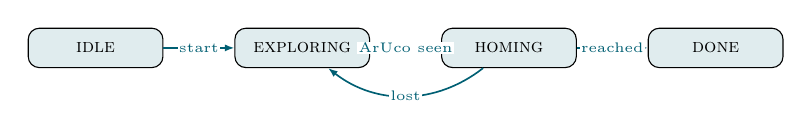
\begin{tikzpicture}[
        font=\scriptsize, node distance=7mm and 9mm,
        st/.style={draw, rounded corners, fill=TealDark!12, minimum height=5mm,
                   inner sep=3pt, text width=1.5cm, align=center},
        e/.style={-{Latex[length=1.2mm]}, semithick, TealDark},
        lbl/.style={font=\tiny, fill=white, inner sep=0.5pt}
      ]
        \node[st] (idle) {\textsc{idle}};
        \node[st, right=of idle] (exp)  {\textsc{exploring}};
        \node[st, right=of exp]  (hom)  {\textsc{homing}};
        \node[st, right=of hom]  (done) {\textsc{done}};
        \draw[e] (idle) -- node[lbl]{start}        (exp);
        \draw[e] (exp)  -- node[lbl]{ArUco seen}   (hom);
        \draw[e] (hom)  -- node[lbl]{reached}      (done);
        \draw[e] (hom)  to[bend left=38] node[lbl]{lost} (exp);
      \end{tikzpicture}
      \end{center}
      \vspace{2pt}

      \textbf{Frontier scoring} (heading-inflated distance):
      \[\text{score}=w_d\,\widehat{\text{prox}}+w_s\,\widehat{\text{area}},
        \quad (w_d,w_s)=(0.85,0.15)\]
      {\small Heading penalty $\bigl(\tfrac{1+\cos\Delta\theta}{2}\bigr)^3$ —
      clusters ${>}60^\circ$ off-heading scaled by $0.01$, suppressing U-turns}

      \vspace{3pt}
      \begin{block}{Homing}
        \footnotesize
        \textbf{ArucoWorldBridge} converts PnP detection $\to$ world-frame pose
        via TF $\to$ forwarded to A$^\star$. Same planner stack as main mission.
      \end{block}

    \column{0.45\textwidth}
      \centering
      % Triangle layout: step1 apex, steps 2--3 side by side below
      \includegraphics[height=0.24\textheight,keepaspectratio]%
        {XIV_D-frontier_exploration_step1.jpeg}\\[1pt]
      \makebox[\linewidth]{%
        \includegraphics[height=0.24\textheight,keepaspectratio]%
          {XIV_D-frontier_exploration_step2.jpeg}\hfill
        \includegraphics[height=0.24\textheight,keepaspectratio]%
          {XIV_D-frontier_exploration_step3.jpeg}}\\[1pt]
      {\scriptsize Explored (pink) expands into unknown (grey);\\
       cyan = frontier cells; robot homes via A$^\star$}

      \vspace{1pt}
      \begin{alertblock}{Safety nets}
        \footnotesize
        Stall watchdog: no \SI{0.05}{m} in \SI{4}{s} $\to$ re-issue goal\\[1pt]
        A$^\star$ fail $\times 2$ $\to$ blacklist cluster\\[1pt]
        Detection lost $\to$ back to \textsc{exploring}
      \end{alertblock}
  \end{columns}
\end{frame}

\begin{frame}{Automatic Emergency Braking (AEB)}
  \presenter{Jorge}
  \begin{columns}[T]
    \column{0.55\textwidth}
      \textbf{Independent safety layer} — decoupled from planning
      \begin{itemize}\small
        \item Blind-spot mask: $[120^\circ,240^\circ]$ excluded
        \item $n{=}5$ consecutive scans with obstacle $\leq\SI{0.3}{\meter}$ $\to$ STOP
        \item Clear after $n$ clean scans
        \item $\tau = n/f_s = 5/15 \approx \SI{333}{\milli\second}$
      \end{itemize}
      \vspace{4pt}
      Safety bound: $d_\text{min} > v\cdot\tau + d_\text{brake}$
      \vspace{4pt}
      \begin{alertblock}{Mission check (Stage 07)}
        \small FSM verifies \texttt{/amr/emergency\_stop} inactive before proceeding
      \end{alertblock}
    \column{0.43\textwidth}
      \begin{block}{Characterization ($N{=}30$ trials)}
        \centering\footnotesize
        \begin{tabular}{@{}lc@{}}
          \toprule
          Metric & Value \\
          \midrule
          Mean response time & 0.34\,s \\
          Stopping distance  & 0.18\,m \\
          True-positive rate & $28/30$ \\
          False triggers (20 min) & $0$ \\
          Recovery rate & $29/30$ \\
          \bottomrule
        \end{tabular}\\
        \vspace{2pt}
        {\scriptsize $v{=}0.30\,\text{m/s}$;\; threshold $0.30\,\text{m}$;\; \SI{15}{\hertz}}
      \end{block}
  \end{columns}
\end{frame}

% ============================================================
\section{Network Security Middleware}

\begin{frame}{Threat Model}
  \presenter{Fredi}
  \centering
  
\includegraphics[width=0.99\textwidth,height=0.80\textheight,keepaspectratio]{XV_D-attack_vectors_and_security.png}\\
  \vspace{4pt}
  {\small Seven attack vectors (top) paired with countermeasures (bottom)}
\end{frame}

\begin{frame}{SecureEnvelope Message Structure}
  \presenter{Fredi}

\centering

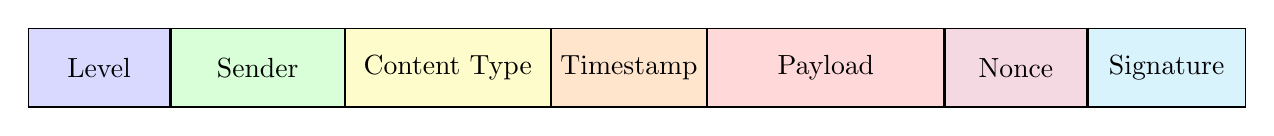
\begin{tikzpicture}[
    box/.style={draw, minimum height=1cm, align=center}
]

\node[box, fill=blue!15, minimum width=1.8cm] (lvl) {Level};

\node[box, fill=green!15, right=0pt of lvl,
      minimum width=2.2cm] (sender) {Sender};

\node[box, fill=yellow!20, right=0pt of sender,
      minimum width=2.6cm] (type) {Content Type};

\node[box, fill=orange!20, right=0pt of type,
      minimum width=1.8cm] (ts) {Timestamp};

\node[box, fill=red!15, right=0pt of ts,
      minimum width=3.0cm] (payload) {Payload};

\node[box, fill=purple!15, right=0pt of payload,
      minimum width=1.8cm] (nonce) {Nonce};

\node[box, fill=cyan!15, right=0pt of nonce,
      minimum width=2.0cm] (sig) {Signature};

\end{tikzpicture}

\vspace{4mm}

\begin{itemize}
\item \textbf{Sender} identifies the publishing node
\item \textbf{Timestamp} enables replay protection
\item \textbf{Payload} contains serialized ROS data
\item \textbf{Nonce} used only for AES-GCM encryption
\item \textbf{Signature} used for RSA-PSS authentication
\end{itemize}

\end{frame}


\begin{frame}{SecureEnvelope Pipeline}
  \presenter{Fredi}
  % Compact TikZ of publish/subscribe flow
  \centering\small
  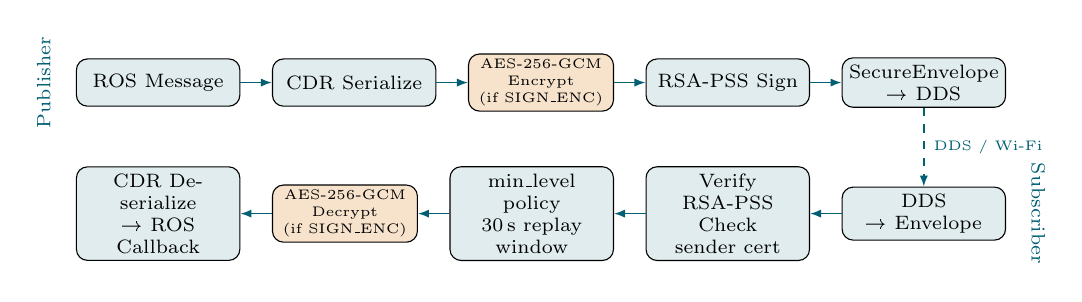
\begin{tikzpicture}[
    font=\scriptsize, node distance=3mm and 4mm,
    box/.style={draw, rounded corners, fill=TealDark!12, align=center,
                inner sep=2.5pt, minimum height=6mm, text width=1.9cm},
    opt/.style={draw, rounded corners, fill=AccentOrange!20, align=center,
                inner sep=2pt, minimum height=5mm, text width=1.7cm, font=\tiny},
    arr/.style={-{Latex[length=1.4mm]}, semithick, TealDark},
    lbl/.style={font=\tiny, above, color=TealDark}
  ]
    % Publisher row
    \node[box] (ros) {ROS Message};
    \node[box, right=of ros] (ser) {CDR Serialize};
    \node[opt, right=of ser] (enc) {AES-256-GCM\\Encrypt\\\tiny(if SIGN\_ENC)};
    \node[box, right=of enc] (sig) {RSA-PSS Sign};
    \node[box, right=of sig] (env) {SecureEnvelope\\→ DDS};

    \draw[arr] (ros)--(ser) node[lbl]{};
    \draw[arr] (ser)--(enc);
    \draw[arr] (enc)--(sig);
    \draw[arr] (sig)--(env);

    % Subscriber row
    \node[box, below=10mm of env] (dds2) {DDS\\→ Envelope};
    \node[box, left=of dds2]  (ver)  {Verify RSA-PSS\\Check sender cert};
    \node[box, left=of ver]   (pol)  {min\_level policy\\30\,s replay window};
    \node[opt, left=of pol]   (dec)  {AES-256-GCM\\Decrypt\\\tiny(if SIGN\_ENC)};
    \node[box, left=of dec]   (deser){CDR Deserialize\\→ ROS Callback};

    \draw[arr] (dds2)--(ver);
    \draw[arr] (ver)--(pol);
    \draw[arr] (pol)--(dec);
    \draw[arr] (dec)--(deser);

    % Down arrow connecting pub to sub
    \draw[arr, dashed] (env.south) -- (dds2.north) node[midway,right,font=\tiny]{DDS / Wi-Fi};

    % Labels
    \node[left=2mm of ros, font=\scriptsize, text=TealDark, rotate=90, anchor=south] {Publisher};
    \node[right=2mm of dds2, font=\scriptsize, text=TealDark, rotate=270, anchor=south] {Subscriber};
  \end{tikzpicture}

  \vspace{6pt}
  \begin{columns}[T]
    \column{0.46\textwidth}
      \begin{block}{PKI}
        \small Self-signed CA (RSA-4096) issues per-node RSA-2048 X.509 certs\\
        AES key $=$ SHA-256(pub-key DER) — no secret distribution
      \end{block}
    \column{0.46\textwidth}
      \begin{alertblock}{Kill switch (NFR-10)}
        \small \texttt{ROS2\_SECURITY\_DISABLED} degrades the entire system uniformly — avoids DDS type mismatch
      \end{alertblock}
  \end{columns}
\end{frame}

\begin{frame}{Secured Communication Topology}
  \presenter{Fredi}
  \centering
  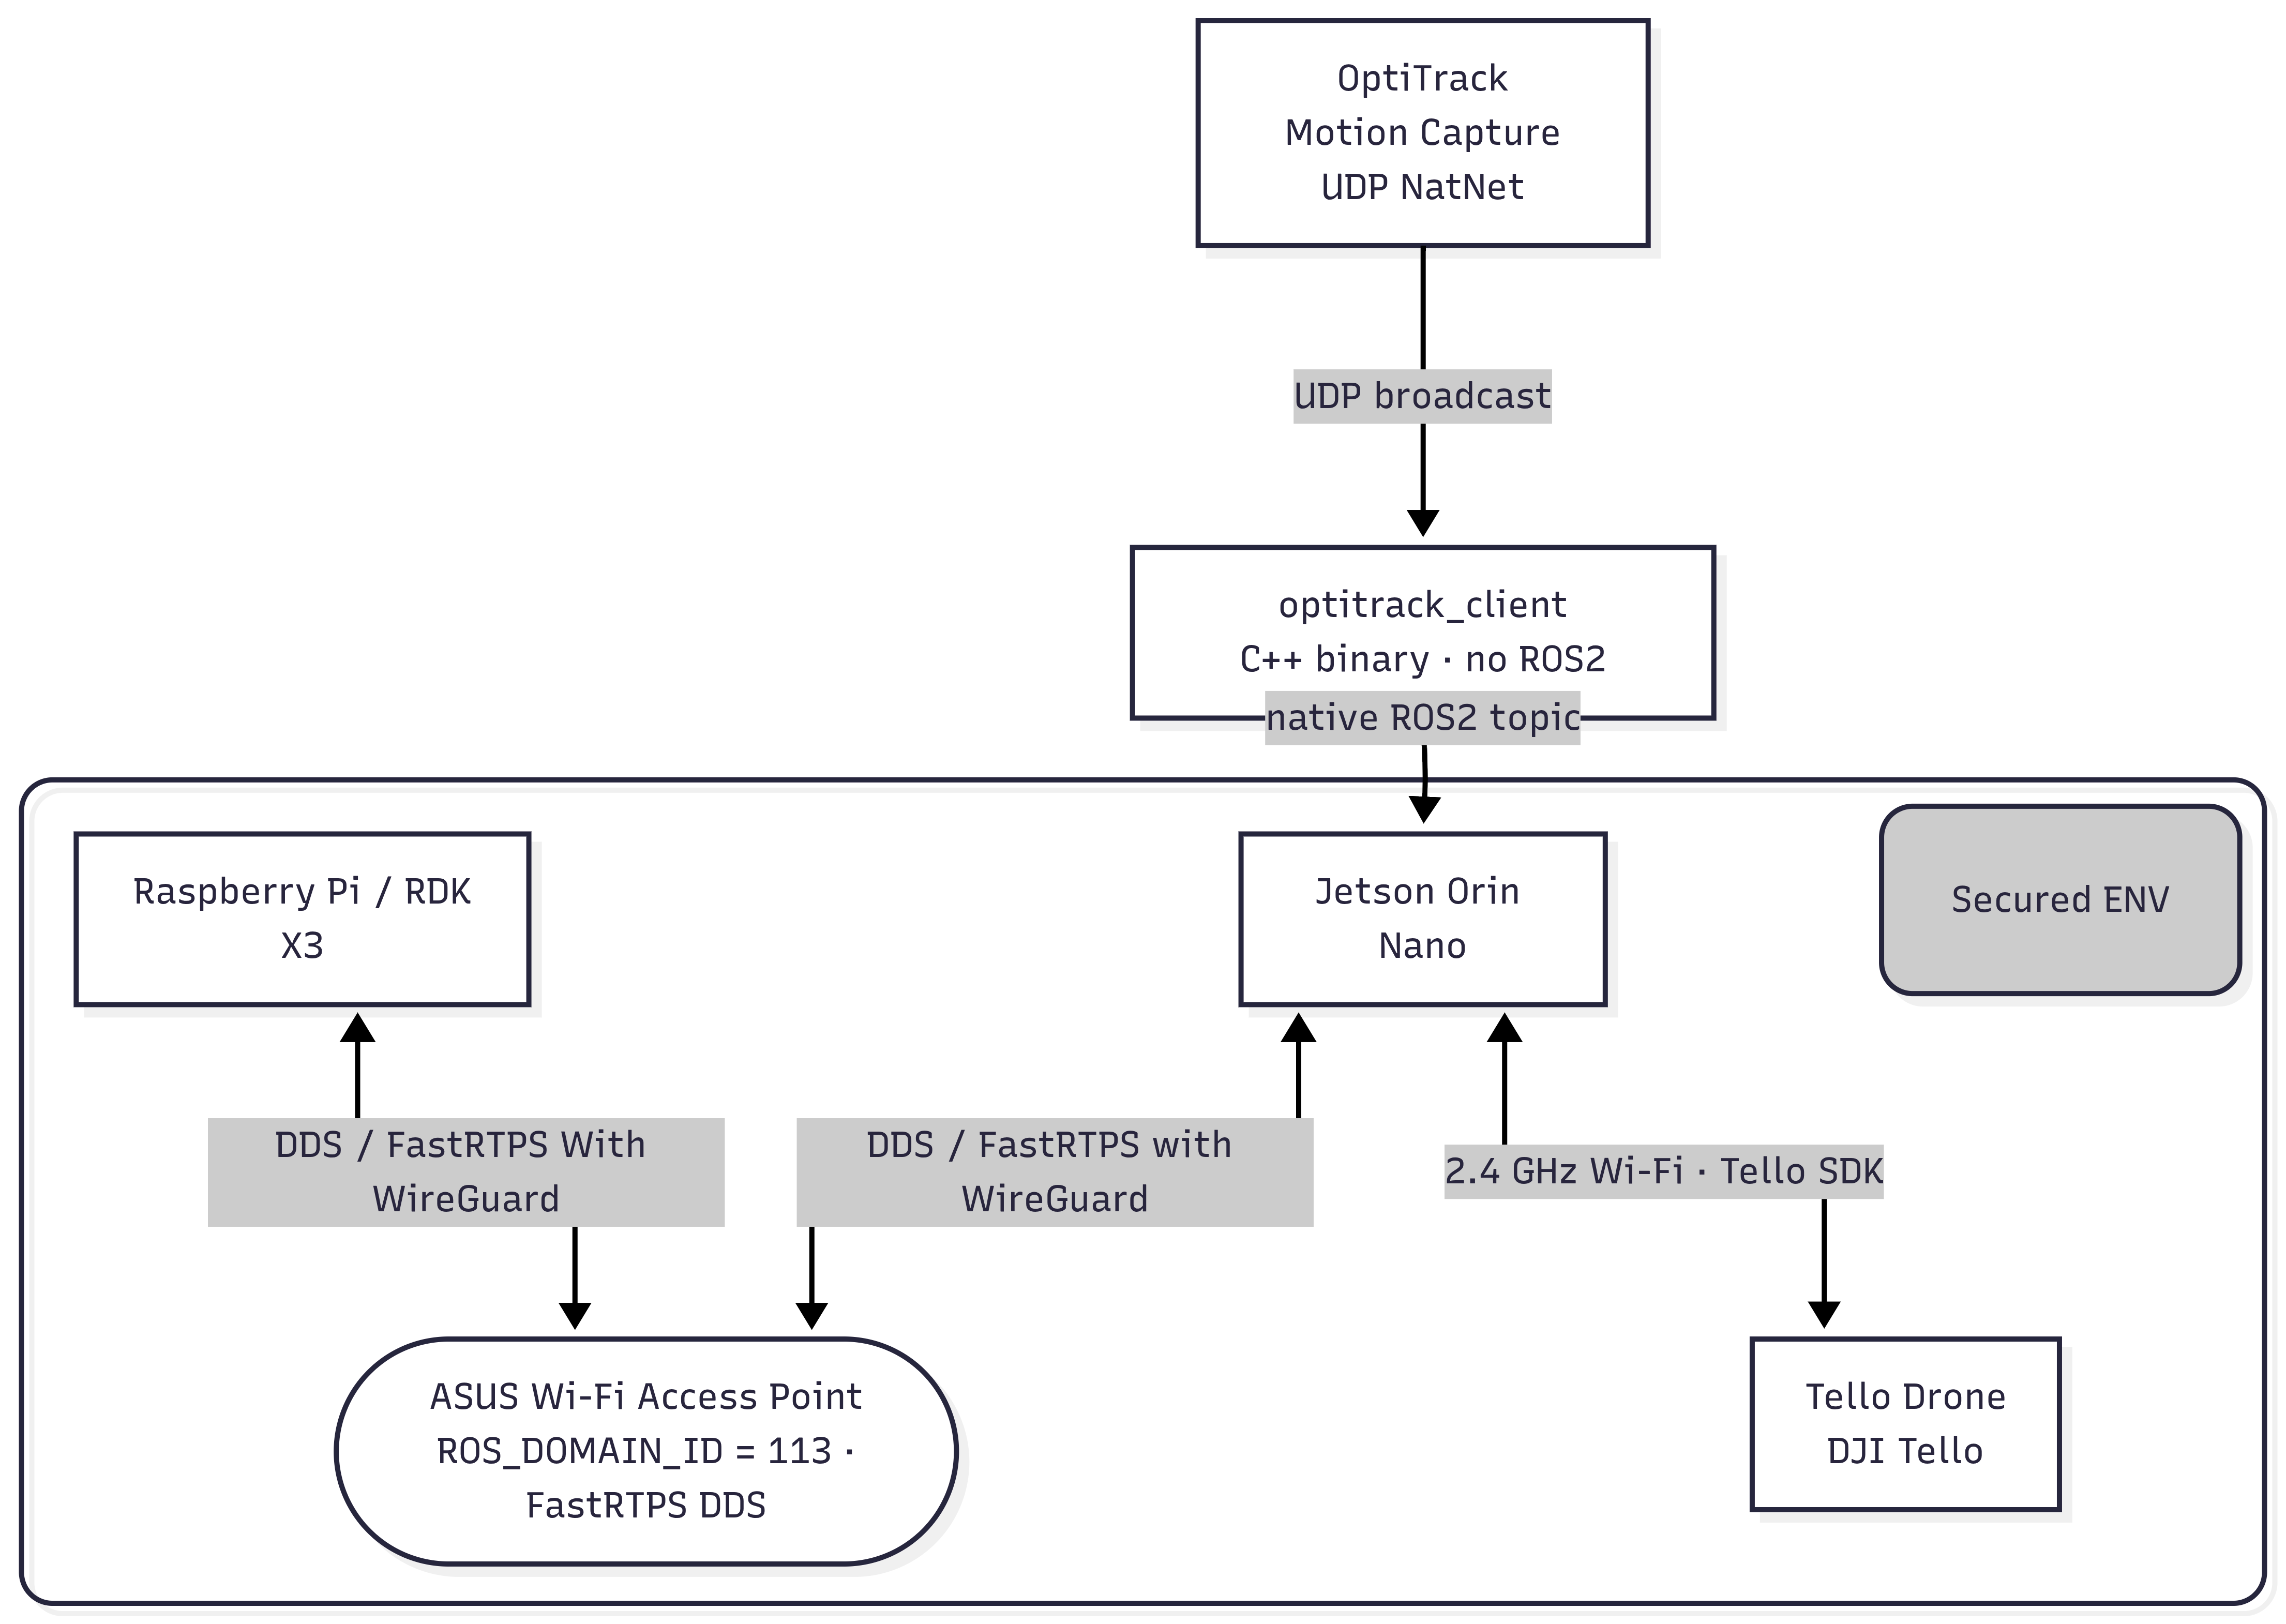
\includegraphics[width=0.95\textwidth,height=0.70\textheight,keepaspectratio]{XV_C-comms_with_security_diagram.png}\\
  \vspace{4pt}
  {\small DDS/FastRTPS over WireGuard-tunnelled Wi-Fi with SecureEnvelope layer.\\
    OptiTrack reaches the robot LAN through a native (non-secured) \texttt{optitrack\_client}.}
\end{frame}

\begin{frame}{Security Overhead: Benchmark Results}
  \presenter{Fredi}
  \begin{columns}[T]
    \column{0.42\textwidth}
      \centering
      \simg{bench_20260612T171805Z_overhead.png}\\
      {\small Per-message cryptographic overhead by level}
    \column{0.56\textwidth}
      \centering
      \simg{bench_20260612T171805Z_latency_overview.png}\\
      {\small End-to-end latency distribution}
  \end{columns}
  \vspace{4pt}
  \begin{block}{Key numbers (small payloads $\leq$\,4\,kB)}
    \footnotesize
    RSA-PSS signing $\approx 10\,\text{ms}$ per message (private-key exponentiation dominates)
    \hfill
    AES-256-GCM adds only $+7$--$11\%$ marginal cost
    \hfill
    Applied selectively to low-frequency mission-critical topics \quad(\textbf{NFR-11 satisfied})
  \end{block}
\end{frame}

% ============================================================
\section{Results and Conclusion}

\begin{frame}{Results Summary}
  \presenter{Jorge}
  \begin{columns}[T]
    \column{0.48\textwidth}
      \textbf{UAV flight control}
      \begin{itemize}\small
        \item Mean tracking error $\leq3.8\,\text{cm}$/axis; RMS $\leq4.4\,\text{cm}$
        \item Within stitching overlap margin
      \end{itemize}
      \medskip
      \textbf{AMR state estimation (EKF)}
      \begin{itemize}\small
        \item Mean $|e_x|{=}4.6\,\text{cm}$, $|e_y|{=}6.3\,\text{cm}$ vs.\ OptiTrack
        \item ${\approx}88\%$ reduction vs.\ wheel odometry alone
      \end{itemize}
      \medskip
      \textbf{Physical safety (AEB)}
      \begin{itemize}\small
        \item $30/30$ true-positive stops at $0.34\,\text{s}$ mean response
        \item Zero false positives in 20 min obstacle-free traversal
      \end{itemize}
    \column{0.50\textwidth}
      \textbf{Security middleware}
      \begin{itemize}\small
        \item All 7 attack-vector suites: 100\% pass
        \item SIGN\_ENCRYPT: ${\sim}10\,\text{ms}$ overhead per message
        \item AES adds only $+7$--$11\%$ over signing alone
        \item Kill switch: 20/20 scenarios validated
      \end{itemize}
      \medskip
      \textbf{System integration}
      \begin{itemize}\small
        \item 12-stage FSM with graceful abort
        \item Map-quality gate: goal-directed or frontier exploration
        \item Decentralized ROS 2 Humble across 3 platforms
      \end{itemize}
  \end{columns}
\end{frame}

\begin{frame}{Conclusion and Future Work}
  \presenter{Jorge}
  \begin{columns}[T]
    \column{0.54\textwidth}
      \textbf{Technical contributions:}
      \begin{itemize}\small
        \item Similarity-transform stitching + learned map-quality gate
        \item From-scratch 5-state EKF with adaptive VIO outlier gate
        \item Robust ArUco localization: geometric median + bias calibration
        \item Registration-free priority-weighted map fusion
        \item Independent streak-detector AEB layer
        \item Application-layer RSA-PSS + AES-256-GCM security middleware
        \item 12-stage orchestrator with graceful PASS/FAIL branching
      \end{itemize}
    \column{0.44\textwidth}
      \textbf{Future work:}
      \begin{itemize}\small
        \item More frequent ArUco re-anchoring (bound dead-reckoning drift)
        \item Online gyro-bias estimation
        \item Dynamic-obstacle prediction in planner
        \item Scale to larger multi-robot teams
        \item Replace RSA sign-per-message with session keys
      \end{itemize}
      \vspace{6pt}
      \begin{block}{Open source}
        \scriptsize
        \texttt{David-OC17/collab\_nav\_ground-jetson}\\
        \texttt{NoeRos22/collab\_nav\_ground-rasp}\\
        \texttt{FrediRomo/security\_middleware}
      \end{block}
  \end{columns}
\end{frame}

\begin{frame}[plain]
  \presenter[TealDark]{David}
  \centering
  \vspace{2.5cm}
  {\LARGE\color{TealDark}\bfseries Thank You}
  \vspace{1.5cm}

  \begin{tabular}{rl}
    \textbf{David Ortiz}      & A01637391@tec.mx \\[2pt]
    \textbf{Alfredo Romo}     & A01643235@tec.mx \\[2pt]
    \textbf{Noé Rosales}      & A00227290@tec.mx \\[2pt]
    \textbf{Sebastian Pulido} & A01642759@tec.mx \\[2pt]
    \textbf{Jorge González}   & A00344893@tec.mx \\
  \end{tabular}
  \vspace{0.8cm}

  {\small In partnership with OMRON Automation and Nuclea Solutions}
\end{frame}

\end{document}
